\textbf{{1.全加器}}

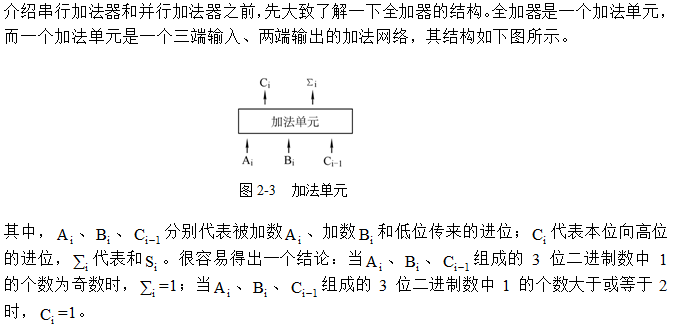
\includegraphics[width=3.69792in,height=1.80208in]{png-jpeg-pics/D212BB742A2C8EB7953DF64B5B055B80.png}

\textbf{{2.串行加法器}}

只设一个全加器的加法器称为串行加法器。两个操作数分别放在两个移位寄存器中,并且由移位寄存器从低位到高位串行地提供操作数进行相加。如果操作数长16位,就需要分成16步进行,每步产生一位和,串行地送入结果寄存器,而产生的进位信号只需要一位触发器,\textbf{每完成一步,用新的进位覆盖旧的进位。}串行加法器的结构如下图所示。

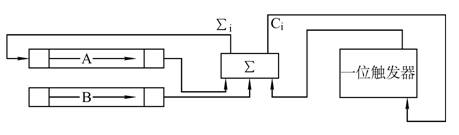
\includegraphics[width=3.69792in,height=1.08333in]{png-jpeg-pics/A79214652D46A367F8629A9938BFE335.png}

\textbf{{3.并行加法器}}

\textbf{(1)并行加法器之串行进位链}

并行加法器由若干个全加器构成,如下图所示。

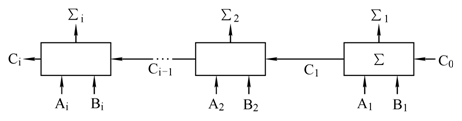
\includegraphics[width=3.69792in,height=0.96875in]{png-jpeg-pics/DDE1F61399F22CA753CD88E3DFBDF8B8.png}

\textbf{(2)并行加法器之并行进位链}

{通常将各位之间传递进位信号的逻辑连接构成的进位线路称为进位链。}{}要想提高运算速度,一定要改善进位链,因此接下来主要从进位链着手来解决问题。

{并行加法器中的进位信号是同时产生的,称为并行进位链。}{并行进位链又分为两种:}\textbf{单重分组跳跃进位链和双重分组跳跃进位链}{。}
